\documentclass[10pt]{article}
\usepackage{graphicx}
\usepackage[margin=1.5cm]{geometry}
\usepackage{amsmath}
\def\brcurs{{\mbox{$\resizebox{.16in}{.08in}{
\includegraphics{BoldR}}$}}}
\def\brcurs{{\mbox{$\resizebox{.16in}{.08in}{
\includegraphics{ScriptR}}$}}}

\begin{document}
\twocolumn

\title{Thursday Warm-up: Vector Algebra Review}
\author{Prof. Jordan C. Hanson}

\maketitle

\section{Review: Vector Algebra}

\begin{enumerate}
\item (a) What is the total distance traveled in Fig. \ref{fig:1} (left), assuming the traveler begins at the origin, and goes North by 4 miles? (b) At the end of the second stage, what is the location of the traveler?  Give both the coordinates and the angle with respect to the x-axis. \\ \vspace{2cm}
\begin{figure}
\centering
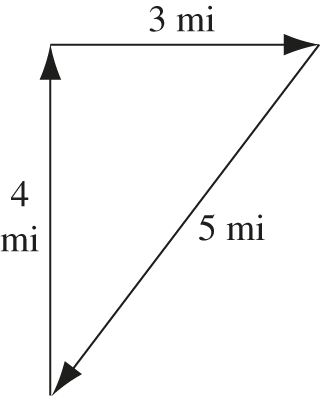
\includegraphics[width=0.2\textwidth]{figures/1_1.jpg} \hspace{0.5cm}
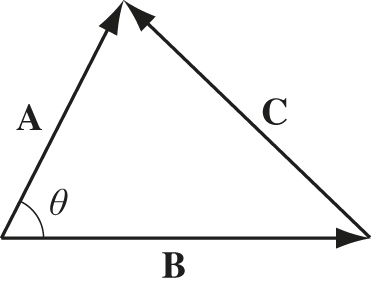
\includegraphics[width=0.2\textwidth]{figures/1_7.jpg}
\caption{\label{fig:1} (Left) A three-stage journey, expressed as vectors. (Right) In this triangle, $\mathbf{A}-\mathbf{B} = \mathbf{C}$.}
\end{figure}
\item Consider Fig. \ref{fig:1} (right).  Let $\mathbf{A}-\mathbf{B} = \mathbf{C}$.  (a) Prove the \textit{law of cosines} by computing $\mathbf{C} \cdot \mathbf{C}$. (b) Suppose $\theta = 90$ degrees.  What is the area of the triangle? \\ \vspace{3cm}
\item (a) Show geometrically that the cross-product $\mathbf{A} \times \mathbf{B}$ in Fig. \ref{fig:2} is equal to the area of the parallelogram. (b) In what direction is the cross-product? \\ \vspace{2cm}
\begin{figure}
\centering
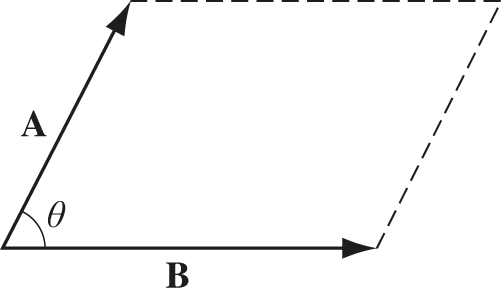
\includegraphics[width=0.33\textwidth]{figures/1_8.jpg}
\caption{\label{fig:2} The magnitude of the cross-product of $\mathbf{A}$ and $\mathbf{B}$ is equal to the area of the parallelogram.}
\end{figure}
\end{enumerate}

\section{Displacement Between Charge and Field Point}

\begin{enumerate}
\item Consider Fig. \ref{fig:3}.  The vector position of a piece of electric charge relative to the origin of the Cartesian coordinate system is $\mathbf{r}'$, and the vector position of the point where we observe the field produced by the charge is $\mathbf{r}$.  (a) Show that the displacement between the charge point and field point is $\brcurs = \mathbf{r}-\mathbf{r}'$. (b) Calculate the magnitude of $\brcurs$ by taking the dot product $\brcurs \cdot \brcurs$, and then taking the square root. (c) Suppose $\mathbf{r} = 5\hat{y} + 4\hat{z}$ cm, and $\mathbf{r}' = 2\hat{y} + 2\hat{z}$ cm.  What is the distance from the charge point to the field point?
\begin{figure}
\centering
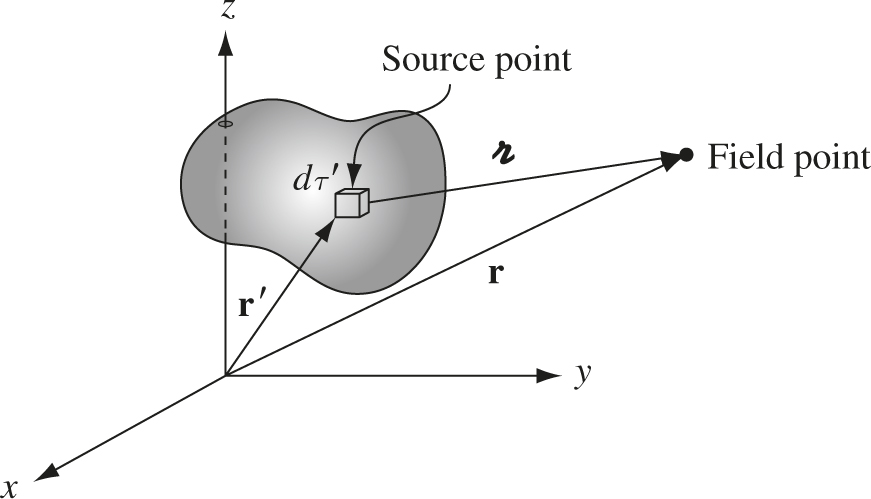
\includegraphics[width=0.4\textwidth]{figures/fm_1.jpg}
\caption{\label{fig:3} The gray region represents a quantity of electric charge, located within a 3D Cartesian coordinate system.}
\end{figure}
\end{enumerate}

\end{document}
